\documentclass[11pt]{article}
\usepackage[margin=2cm,a4paper]{geometry}
\usepackage{graphicx}
\usepackage{authblk}
\usepackage{url}
\usepackage{array}
\usepackage{amsfonts}
\usepackage{multirow}
\usepackage{amsmath}
\usepackage[usenames, dvipsnames]{color, colortbl}
\usepackage[normalem]{ulem}

\usepackage[outdir=./img/]{epstopdf}
\usepackage{epsfig}

\usepackage{tikz}
\usetikzlibrary{fit,positioning}
\usetikzlibrary{arrows}

\makeatletter
\def\title#1{\gdef\@title{Supplement to: ``#1''}}
\makeatother
\renewcommand{\thetable}{S\arabic{table}}%
\renewcommand{\thefigure}{S\arabic{figure}}%
\renewcommand{\thepage}{S\arabic{page}}

\setlength\parindent{0pt}


% supplement referencing
\usepackage{subcaption}
%\usepackage{cleveref}

% tablet style table
 \usepackage{booktabs}
 
\title{Triqler for Protein Summarization of Data from Data Independent Aquisition Mass Spectrometry}
\author{Patrick Truong \and Matthew The \and Lukas K\"{a}ll}


\begin{document}

\maketitle

\section*{Note S1: Supplementary figures and tables}
\label{sec:fc-eval}

\section*{Supplementary Tables}

\begin{table}[h]
    \begin{tabular}{lllllll}
    \hline
    \multicolumn{7}{c}{ID workflow}                                                                                                                                                                                   \\ \hline
    Condition & \multicolumn{3}{c}{1}                                                                         & \multicolumn{3}{c}{2}                                                                         \\
    Run       & \multicolumn{1}{c}{002-Pedro} & \multicolumn{1}{c}{004-Pedro} & \multicolumn{1}{c}{006-Pedro} & \multicolumn{1}{c}{003-Pedro} & \multicolumn{1}{c}{005-Pedro} & \multicolumn{1}{c}{007-Pedro} \\
    Peptides  & 20 747                        & 21 445                        & 21 016                        & 20 494                        & 22 792                        & 22 787                        \\
    Proteins  & 2 836                         & 2 857                         & 2 869                         & 2 818                         & 2 909                         & 2 918                         \\ \hline
    \end{tabular}
     \caption{{\bf Number of identified peptides and proteins for the samples using the ID workflow.}
          \label{fig:osw_peptide_and_protein_id}}
\end{table}
        

\begin{table}[h]
    \begin{tabular}{lllllll}
    \hline
    \multicolumn{7}{c}{PS workflow}                                                                                                                                                                                   \\ \hline
    Condition & \multicolumn{3}{c}{1}                                                                         & \multicolumn{3}{c}{2}                                                                         \\
    Run       & \multicolumn{1}{c}{002-Pedro} & \multicolumn{1}{c}{004-Pedro} & \multicolumn{1}{c}{006-Pedro} & \multicolumn{1}{c}{003-Pedro} & \multicolumn{1}{c}{005-Pedro} & \multicolumn{1}{c}{007-Pedro} \\
    Peptides  & 21 036                        & 20 783                        & 21 040                        & 21 243                        & 21 325                        & 21 248                        \\
    Proteins  & 3 377                         & 3 350                         & 3 368                         & 3 358                         & 3 381                         & 3 356                         \\ \hline
    \end{tabular}
     \caption{{\bf Number of identified peptides and proteins for the samples using the PS workflow.}
          \label{fig:diann_peptide_and_protein_id}}
\end{table}

\iffalse
\subsection*{Fold change distributions}
\begin{figure}[hbt]
    \centering
    \begin{tabular}{lclc} 
        A & 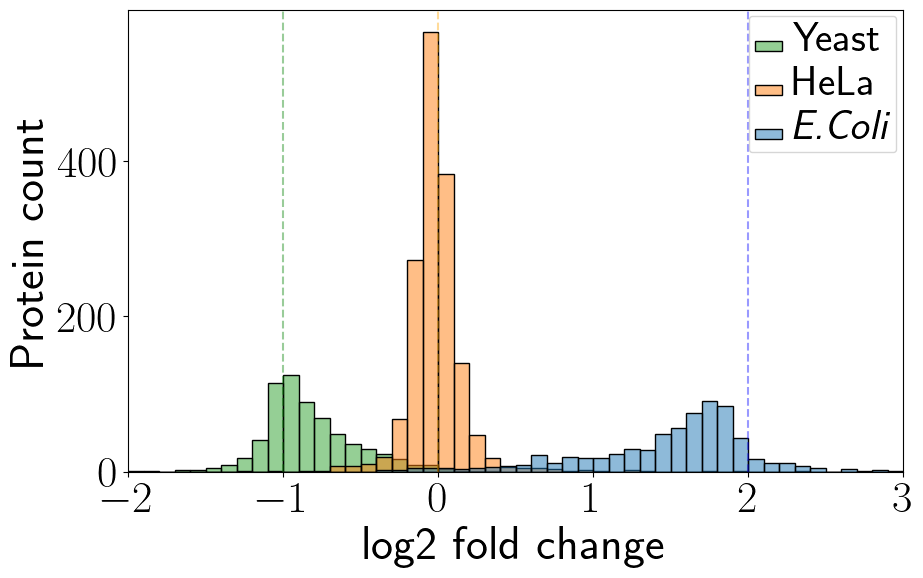
\includegraphics[width=0.4\linewidth]{../../result/report_plots_pipeline/histogram_ID_triqler.png} & 
        E & 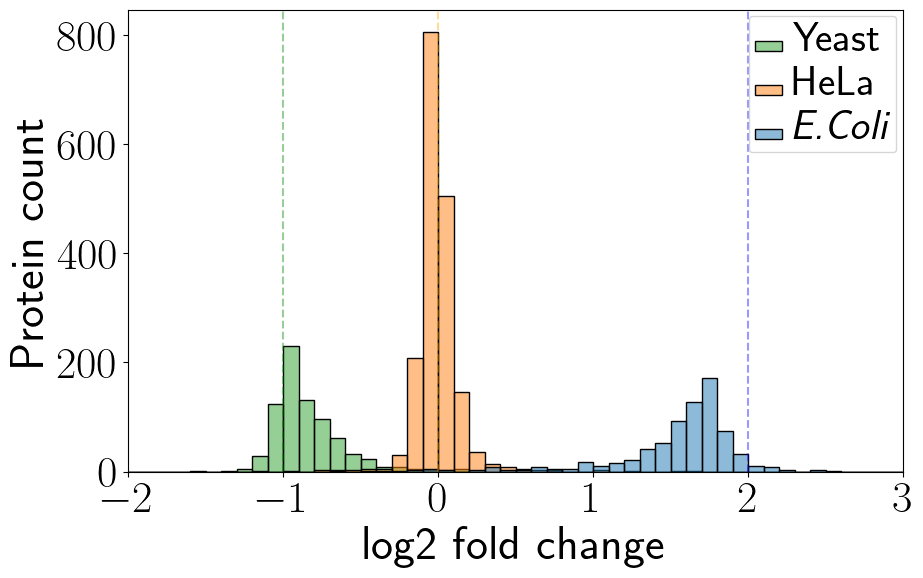
\includegraphics[width=0.4\linewidth]{../../result/report_plots_pipeline/histogram_PS_triqler.png} \\ 
        B & 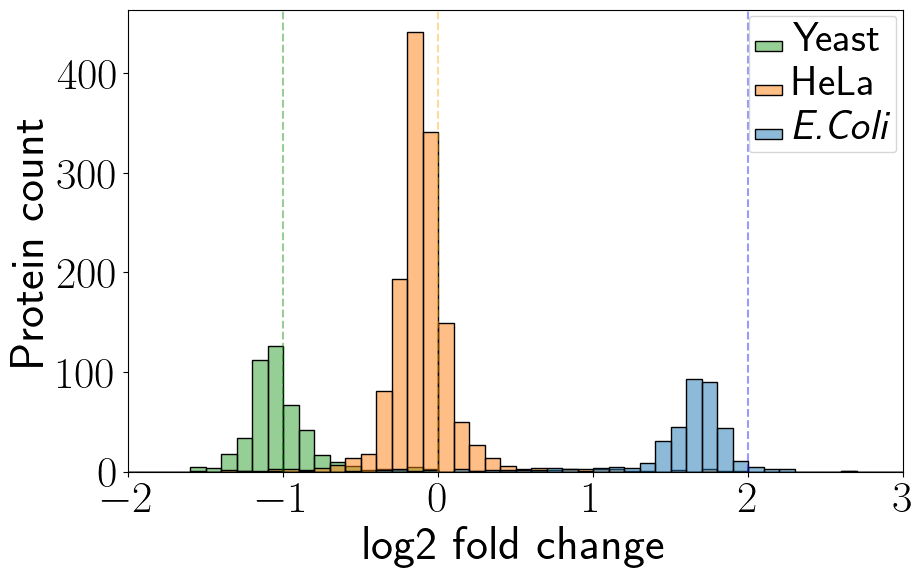
\includegraphics[width=0.4\linewidth]{../../result/report_plots_pipeline/histogram_ID_msqrob2.png} & 
        F & 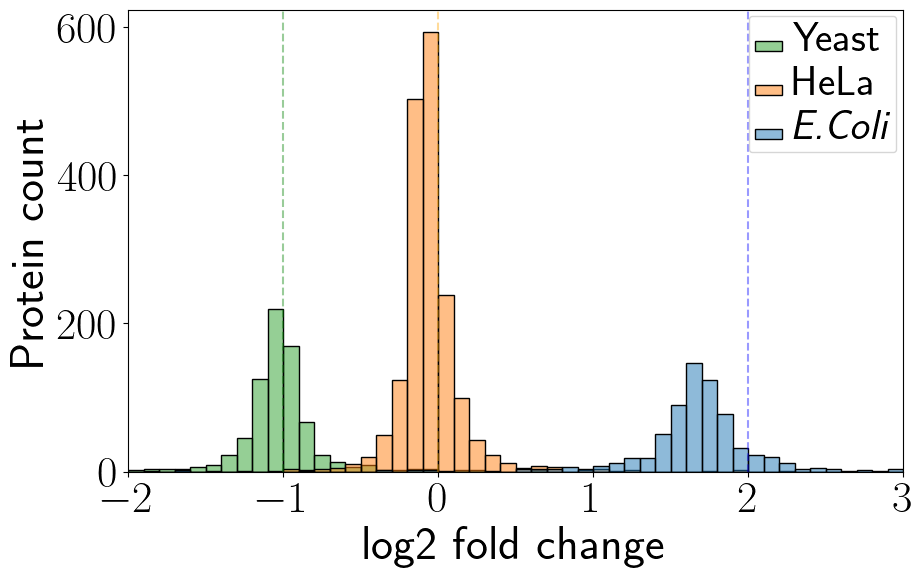
\includegraphics[width=0.4\linewidth]{../../result/report_plots_pipeline/histogram_PS_msqrob2.png} \\ 
        C & 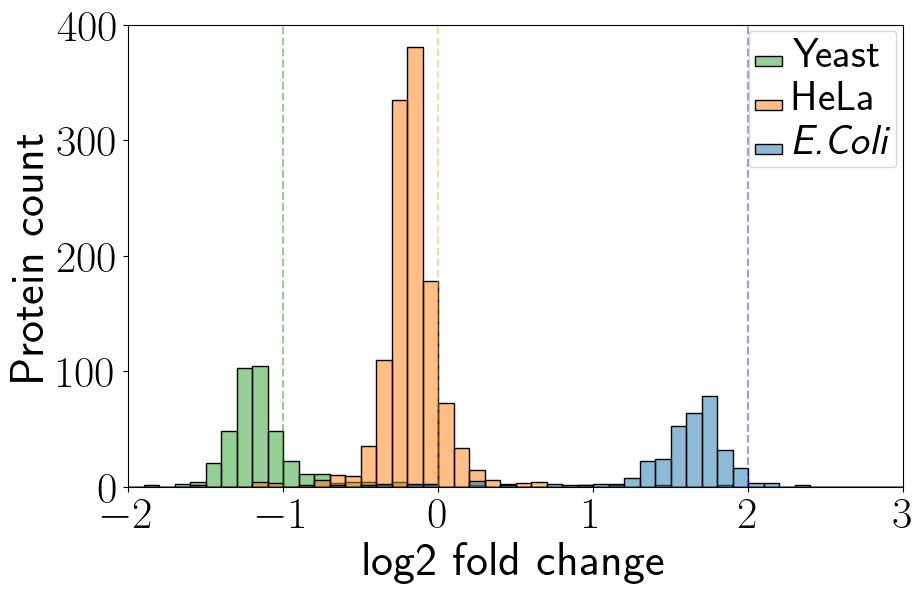
\includegraphics[width=0.4\linewidth]{../../result/report_plots_pipeline/histogram_ID_msstats.png} & 
        G & 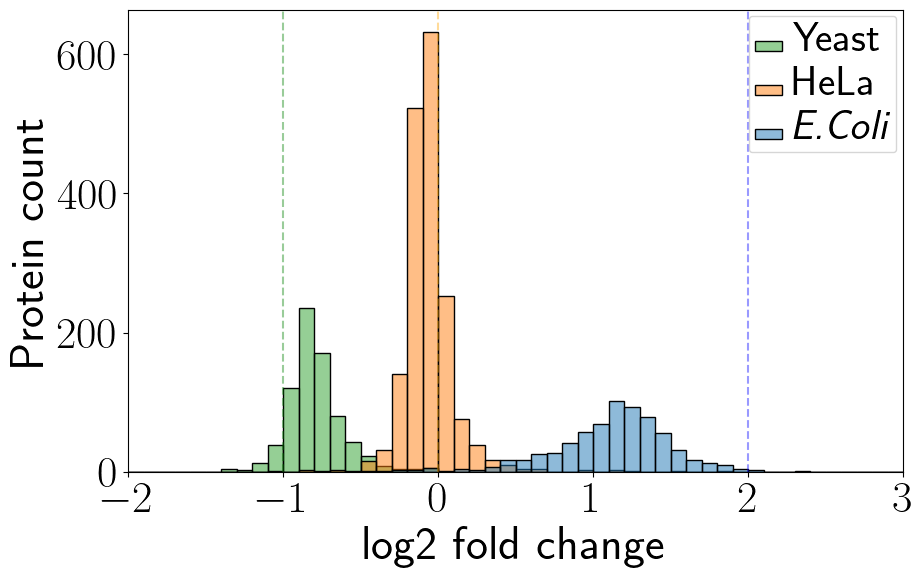
\includegraphics[width=0.4\linewidth]{../../result/report_plots_pipeline/histogram_PS_msstats.png} \\ 
        D & 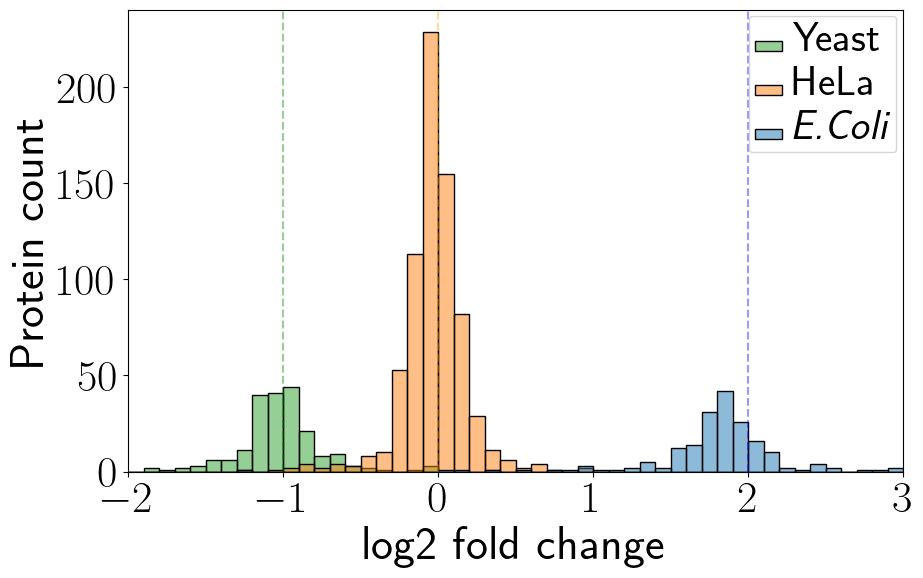
\includegraphics[width=0.4\linewidth]{../../result/report_plots_pipeline/histogram_ID_top3.png} &
        H & 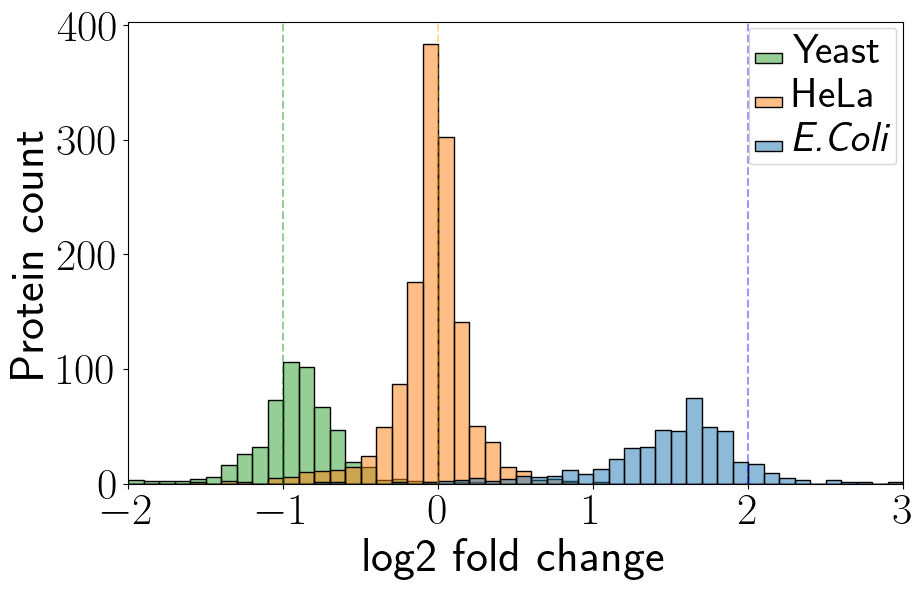
\includegraphics[width=0.4\linewidth]{../../result/report_plots_pipeline/histogram_PS_top3.png} 
    \end{tabular}
   
    \caption{{\bf Comparison of reported fold change distributions.} We used protein data from (A-D) ID pipeline and (E-H) PS pipeline as generated by 
    (A,E) Triqler, (B,F) MSqRob2, (C,G) MSstats, and (D,H) Top-3. For these histograms we included all the summarized proteins, and did not remove any proteins based on significance or fold-change treshholds.  \label{fig:fc_histogram_again}}
\end{figure}

\fi




\subsubsection*{Comparison of ability to differentiate differentially abundant proteins}
\begin{figure}[hbt]
    \centering
    \begin{tabular}{lclc} 
        A & \includegraphics[width=0.4\linewidth]{../../result/report_plots_pipeline/diff_HeLa_vs_nonHeLa_ID_ecoli_051.png} & 
        D & \includegraphics[width=0.4\linewidth]{../../result/report_plots_pipeline/diff_HeLa_vs_nonHeLa_PS_ecoli_051.png} \\ 
        B & \includegraphics[width=0.4\linewidth]{../../result/report_plots_pipeline/diff_HeLa_vs_nonHeLa_ID_yeast_051.png} & 
        E & \includegraphics[width=0.4\linewidth]{../../result/report_plots_pipeline/diff_HeLa_vs_nonHeLa_PS_yeast_051.png} \\
        C & \includegraphics[width=0.45\linewidth]{../../result/report_plots_pipeline/diff_HeLa_vs_nonHeLa_ID_all_051.png} & 
        F & \includegraphics[width=0.45\linewidth]{../../result/report_plots_pipeline/diff_HeLa_vs_nonHeLa_PS_yeast_051.png} \\ 

    \end{tabular}
    \caption{{\bf Comparison of ability to differentiate differentially abundant proteins} We plotted the number of reported differentially abundant  {\em E. Coli} and Yeast proteins as a function of number of proteins from the HeLa background when sorting according to significance for (A) SL pipeline and (B) PS pipeline. For the test we selected a fold-change evaluation of 0.51 for Triqler and fold-change treshold of 0.51 for Top3, MSstats and MSqRob2. All methods have an protein-level FDR threshold of 0.01. \label{fig:ability_to_differentiate_differentially_abundant_specie_vs_hela}}
\end{figure}

\iffalse
\subsubsection*{Differential abundance, as reported by each protein summarization method}
\begin{figure}[hbt]
    \centering
    \begin{tabular}{lclc} 
        A & 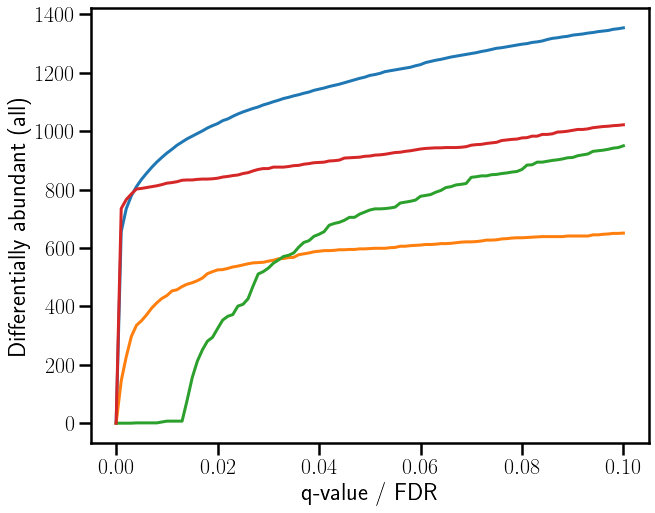
\includegraphics[width=0.4\linewidth]{../../result/report_plots_filtered/osw_de_all.png} & 
        E & 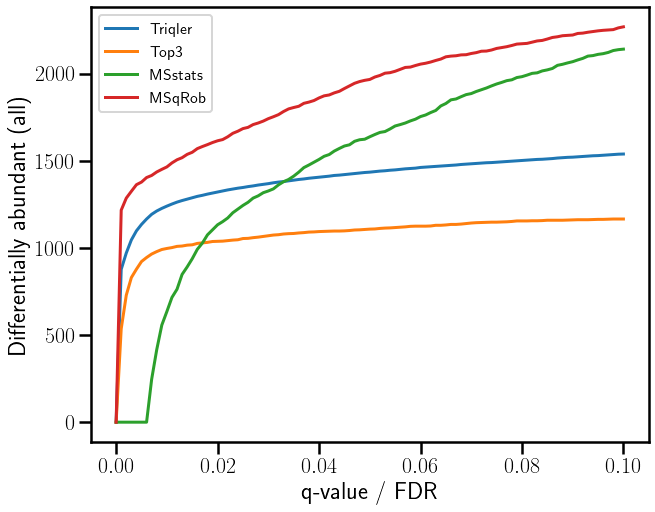
\includegraphics[width=0.4\linewidth]{../../result/report_plots_filtered/diann_de_all.png} \\ 
        B & 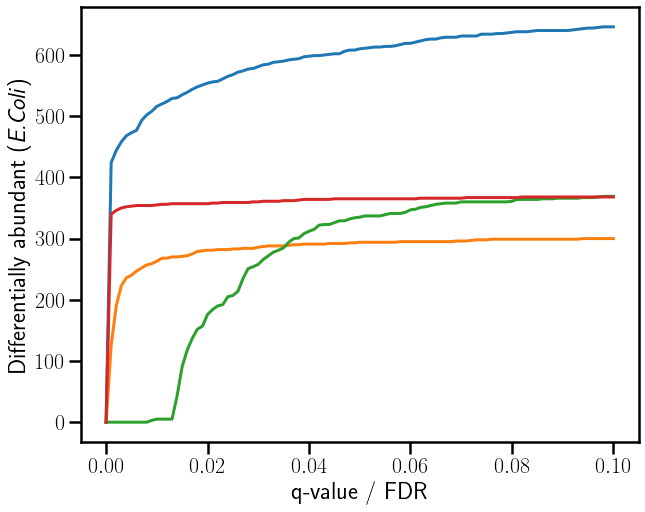
\includegraphics[width=0.4\linewidth]{../../result/report_plots_filtered/osw_de_ecoli.png} & 
        F & 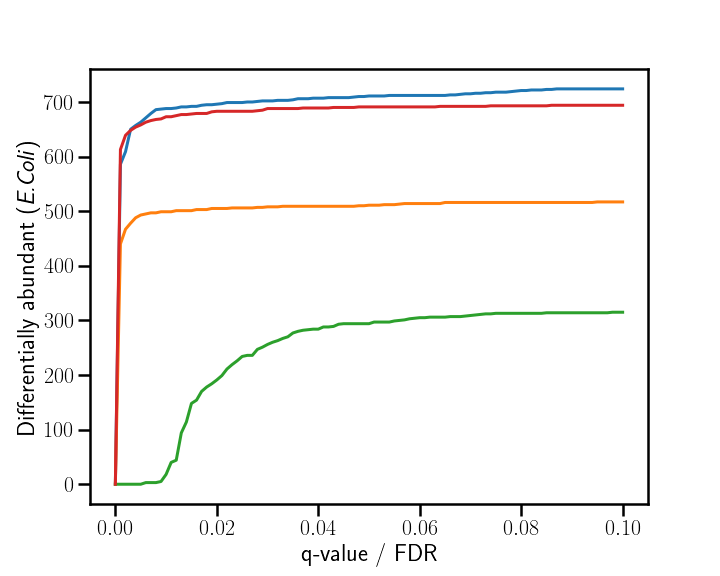
\includegraphics[width=0.4\linewidth]{../../result/report_plots_filtered/diann_de_ecoli.png} \\ 
        C & 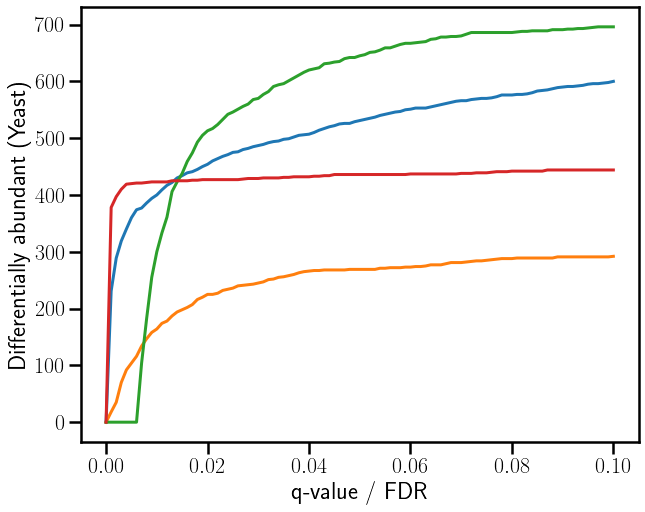
\includegraphics[width=0.4\linewidth]{../../result/report_plots_filtered/osw_de_yeast.png} & 
        G & 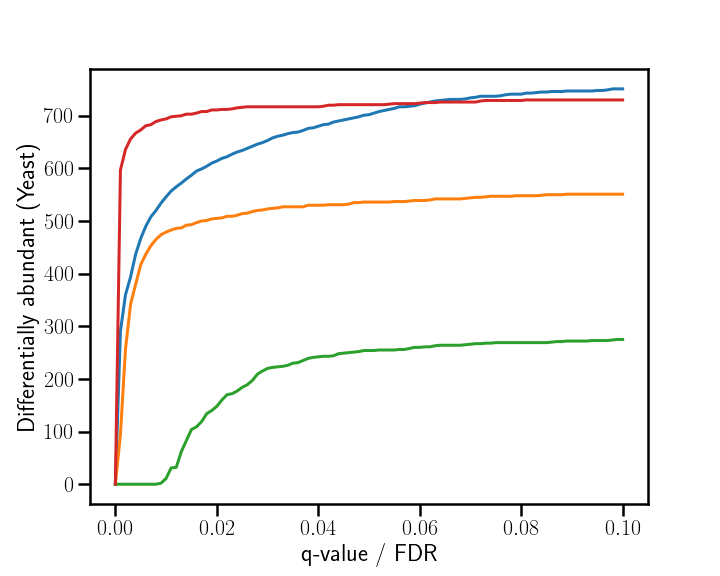
\includegraphics[width=0.4\linewidth]{../../result/report_plots_filtered/diann_de_yeast.png} \\ 
        D & 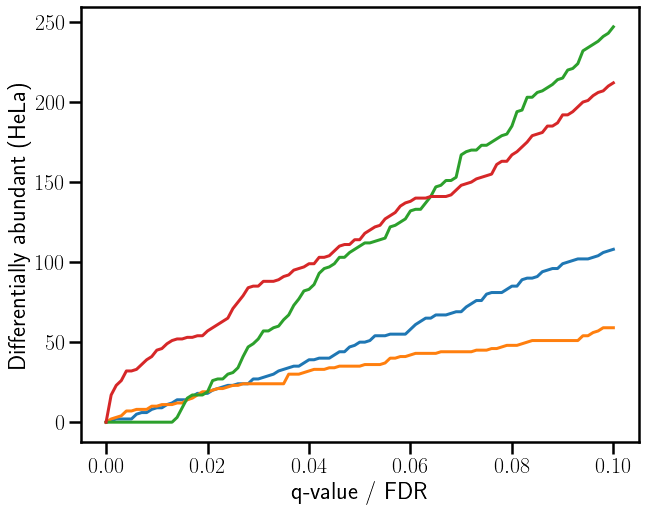
\includegraphics[width=0.4\linewidth]{../../result/report_plots_filtered/osw_de_human.png} &
        H & 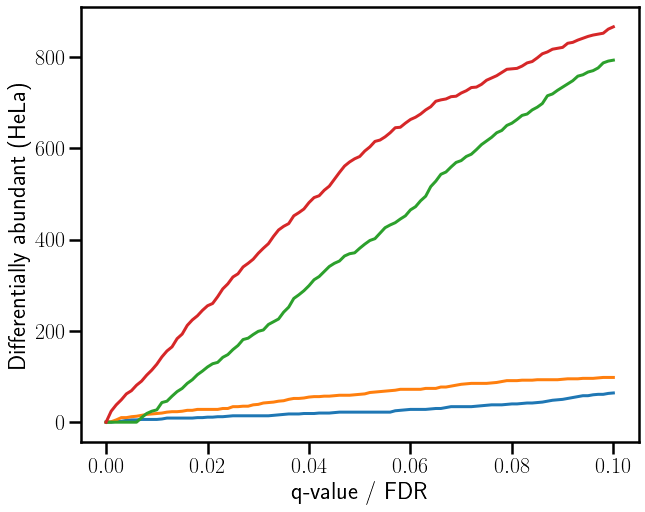
\includegraphics[width=0.4\linewidth]{../../result/report_plots_filtered/diann_de_human.png} 
        A 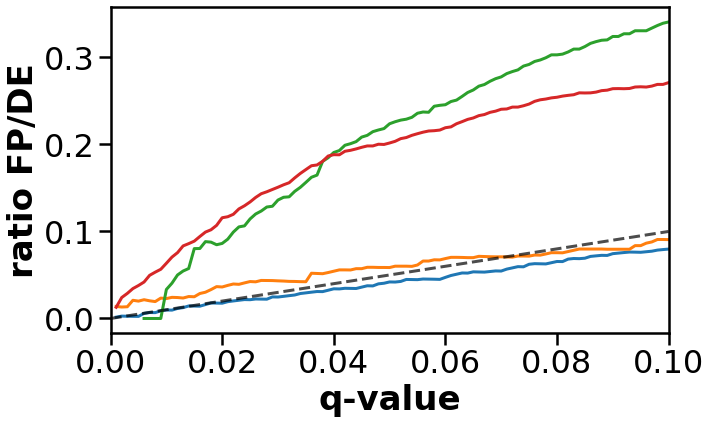
\includegraphics[width=0.5\linewidth]{../../result/report_plots/osw_FP_DE_all.png} & &%\includegraphics[width=0.3\linewidth]{} & 
        B 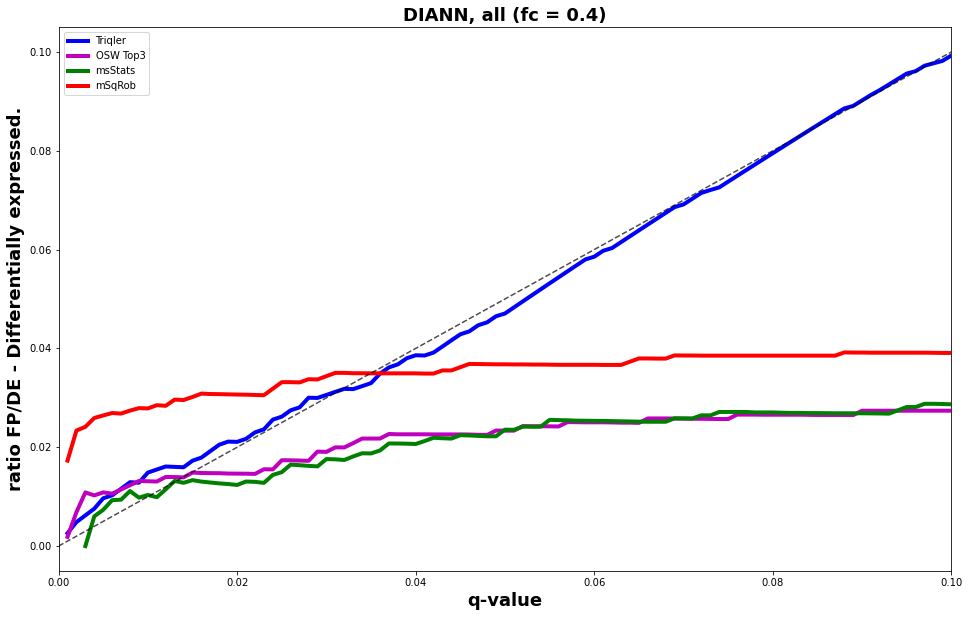
\includegraphics[width=0.5\linewidth]{../../result/report_plots/diann_FP_DE_all.png} & \\%\includegraphics[width=0.3\linewidth]{} \\
    \end{tabular}
    \caption{{\bf Comparison of reported differential abundance.} Here we plotted the number of reported differentially abundant proteins as a function of each methods reported error estimate. In (A-D) results from the SL pipeline and in (E-H) PS pipeline were used. 
    (A,E) All, (B,F) \textit{E.Coli}, (C,G) yeast, and (D,H) HeLa. \label{fig:da_methods_esimate}}
    %TODO: what is meant with this? E.g. did you only consider coli proteins for generating B? 
\end{figure}
\fi


\iffalse
\subsubsection*{Comparison of statistical calibration}
\begin{figure}[hbt]
    \centering
    \centering
    \begin{tabular}{lclc} 
        %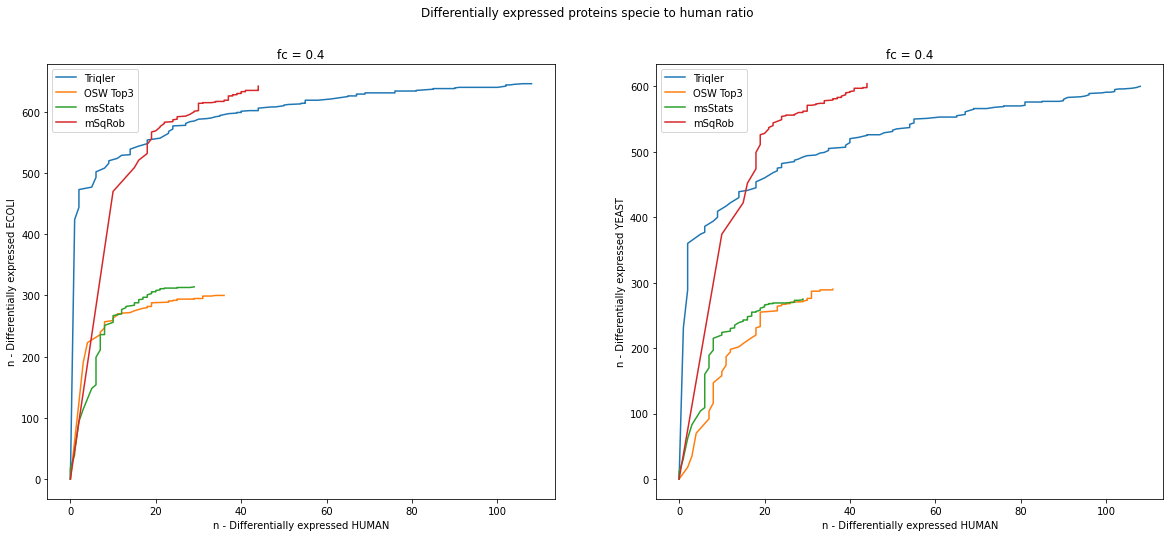
\includegraphics[width=0.3\linewidth]{../../result/report_plots/de_human_vs_de_specie.png} & 
        %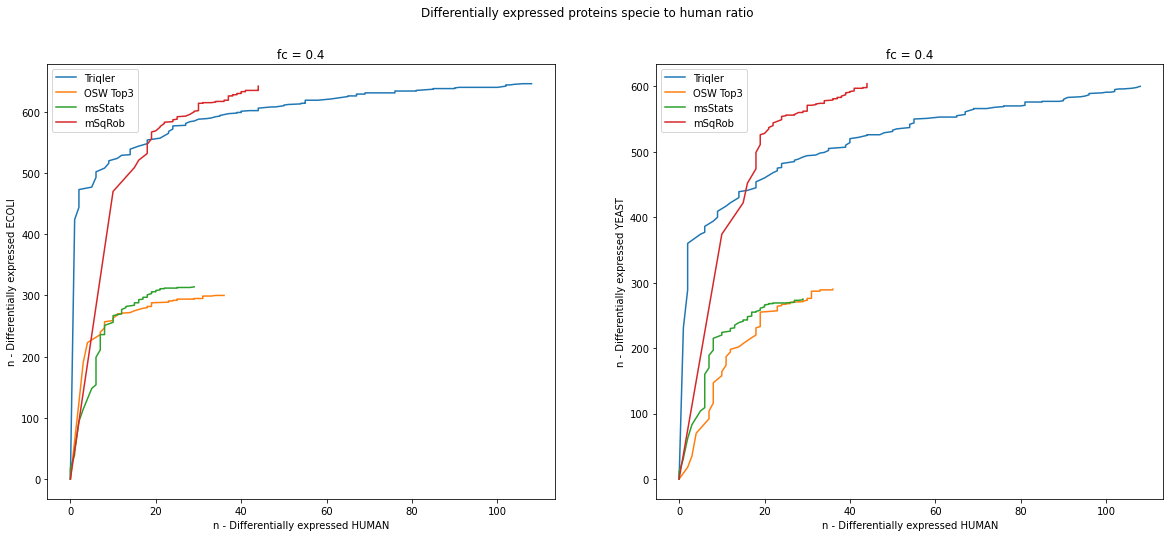
\includegraphics[width=0.3\linewidth]{../../result/report_plots/de_human_vs_de_specie.png} \\ 
        %A & B
        % A 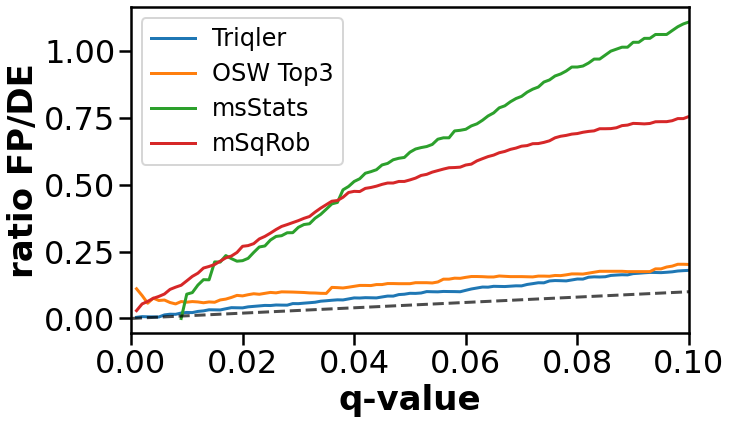
\includegraphics[width=0.5\linewidth]{../../result/report_plots/osw_FP_DE_yeast.png} & &%\includegraphics[width=0.3\linewidth]{} & 
        % D 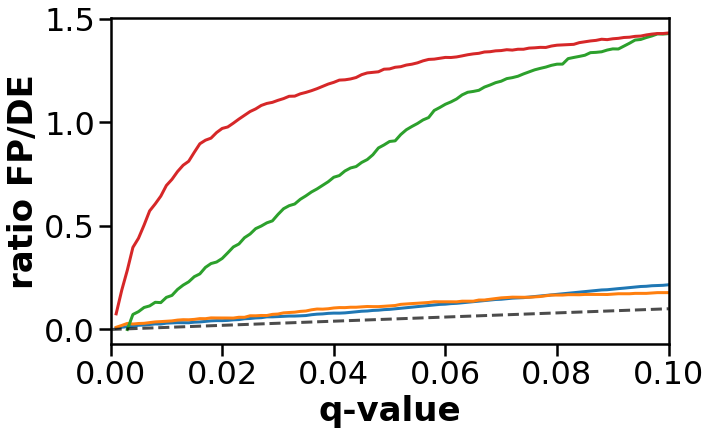
\includegraphics[width=0.5\linewidth]{../../result/report_plots/diann_FP_DE_yeast.png} & \\%\includegraphics[width=0.3\linewidth]{} \\ 
        % B 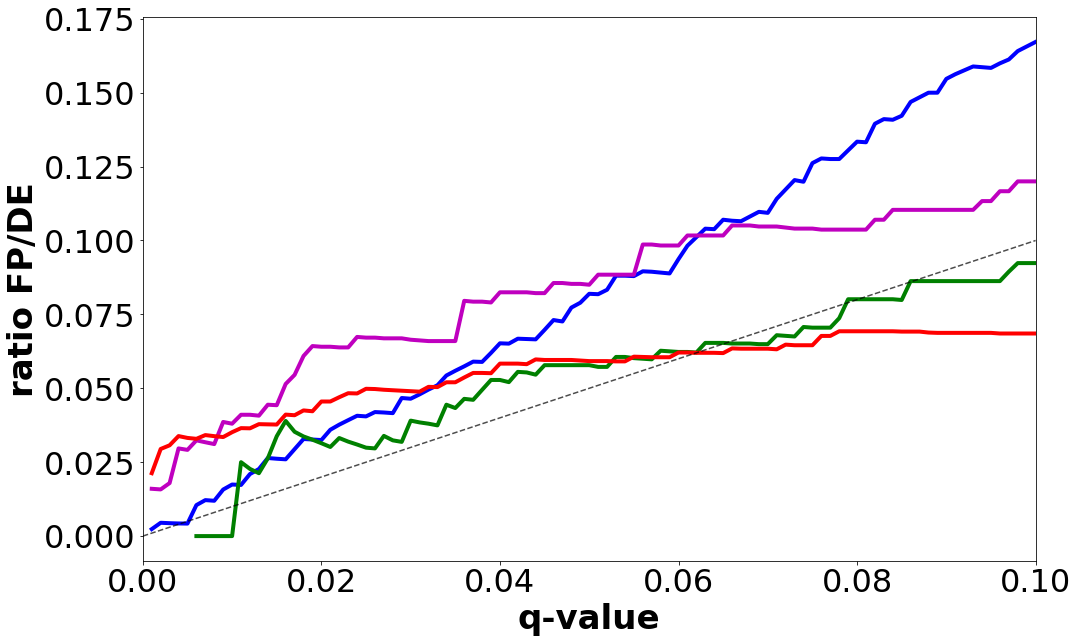
\includegraphics[width=0.5\linewidth]{../../result/report_plots/osw_FP_DE_ecoli.png} & &%\includegraphics[width=0.3\linewidth]{} & 
        % E 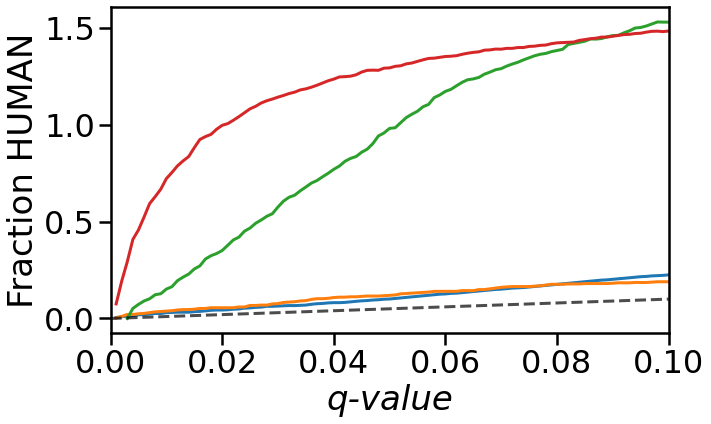
\includegraphics[width=0.5\linewidth]{../../result/report_plots/diann_FP_DE_ecoli.png} & \\%\includegraphics[width=0.3\linewidth]{} \\ 
        A 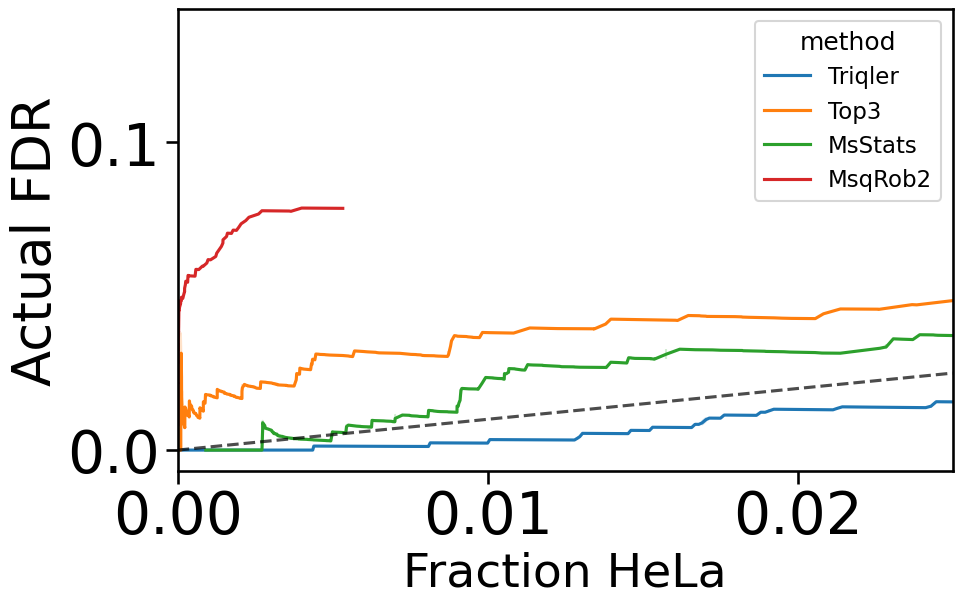
\includegraphics[width=0.5\linewidth]{../../result/report_plots_pipeline/calibration_ID_0.48.png} & &%\includegraphics[width=0.3\linewidth]{} & 
        B 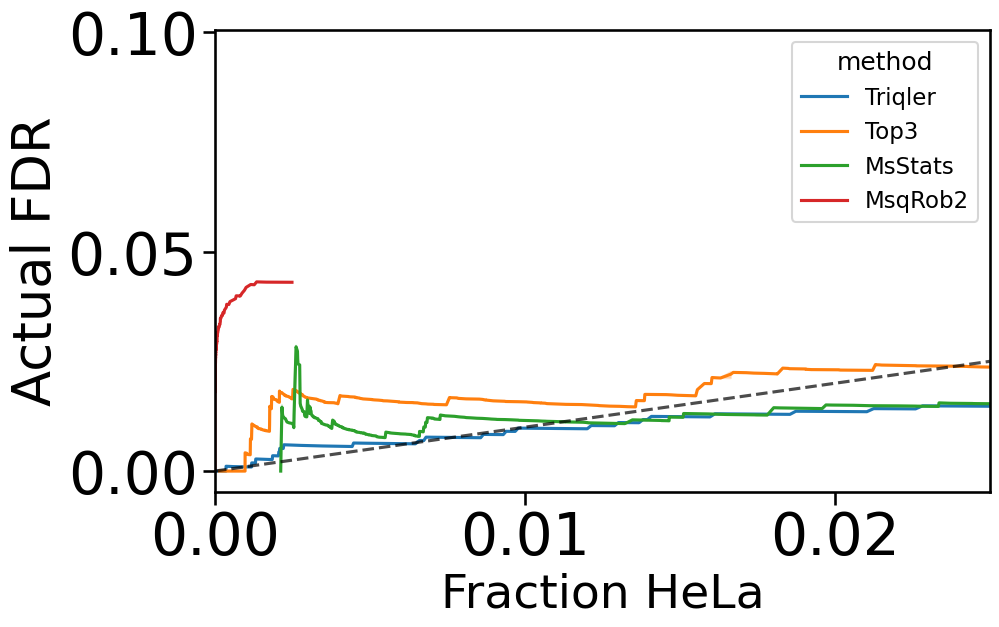
\includegraphics[width=0.5\linewidth]{../../result/report_plots_pipeline/calibration_PS_0.48.png} & \\%\includegraphics[width=0.3\linewidth]{} \\ 
    \end{tabular}
  \caption{{\bf Comparison of calibration of the compared summarization methods.} We plotted the fraction of reported differentially abundant HeLa proteins as a function of $q$~value for (A) ID pipeline and (B) PS pipeline. \label{fig:frac_hela_vs_fdr}}
\end{figure}
\fi

\subsubsection*{Constant variance}
\begin{figure}[hbt]
    \centering
    \centering
    \begin{tabular}{lclc} 
        A 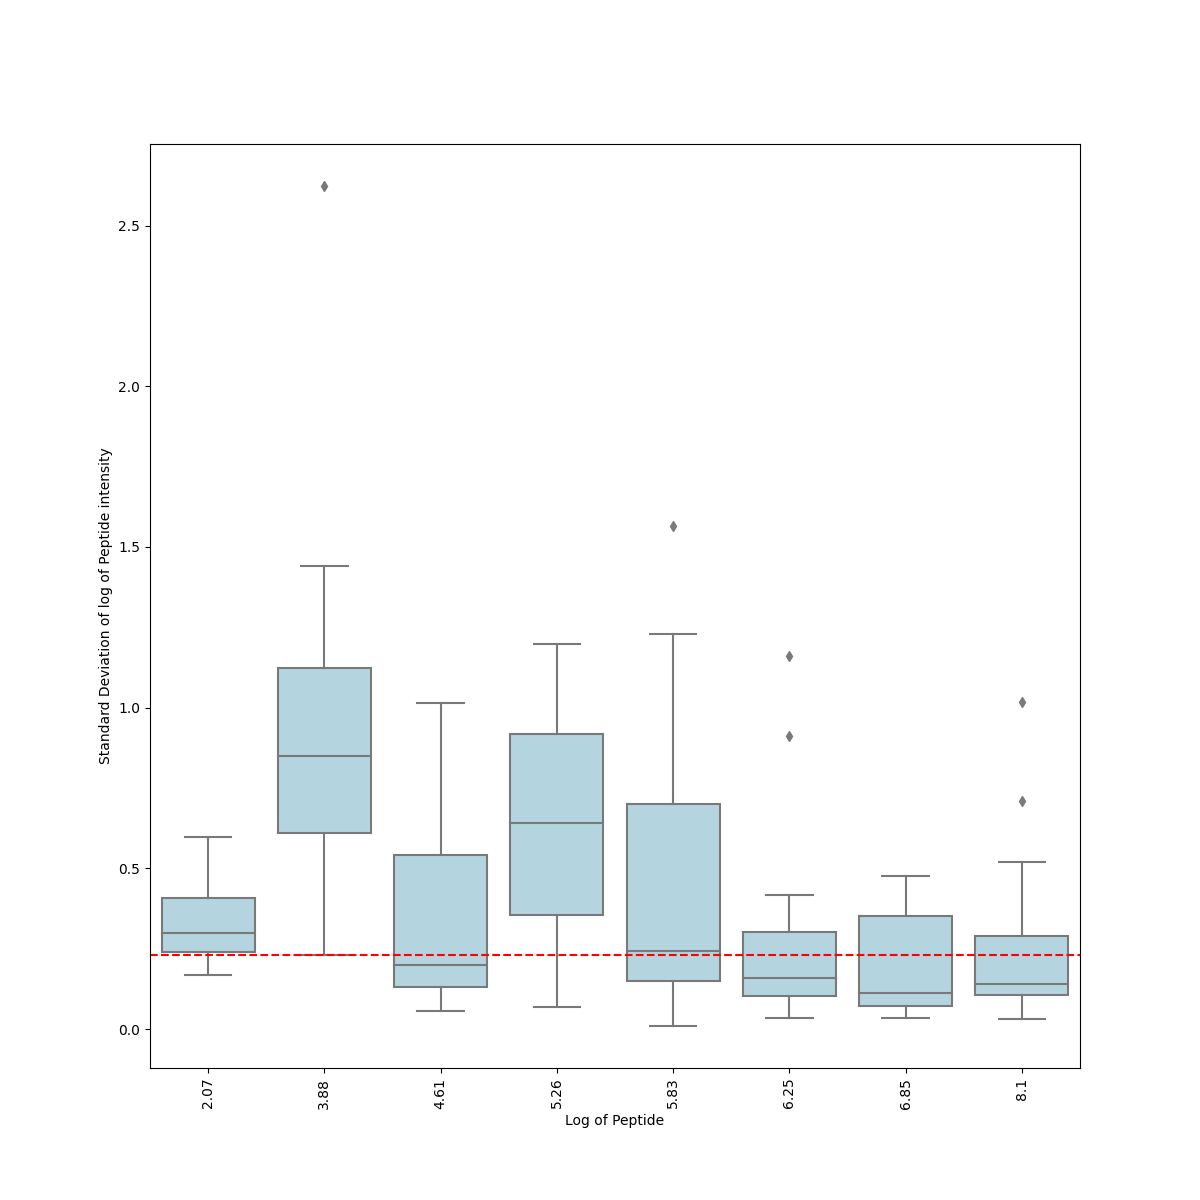
\includegraphics[width=0.5\linewidth]{../../result/report_plots_pipeline/quantile_bins_ID_median.png} & &
        B 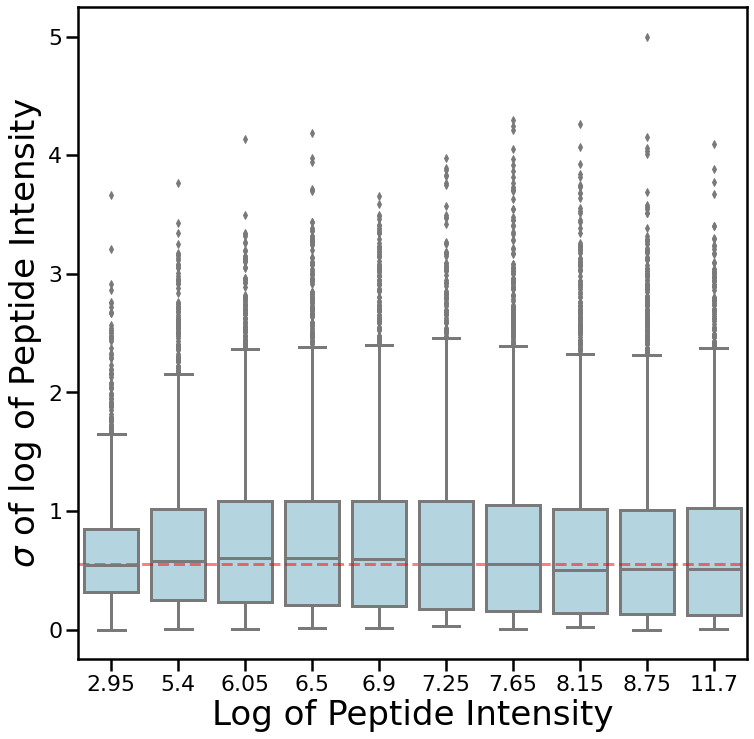
\includegraphics[width=0.5\linewidth]{../../result/report_plots_pipeline/quantile_bins_PS_median.png} & \\
    \end{tabular}
  \caption{{\bf Uniform offset in standard deviation.} We plotted the standard deviation as a function of the mean of every peptide intensity in the TripleTOF6600 section of the LFQ Bench set  in a log-log scale for (A) ID pipeline and (C-D) PS pipeline.  We observe a nearly uniform offset in standard deviation across the intensity scale, demonstrating that $\log(\sigma) \approx \log(\mu) + \log(k)$ and hence   $\sigma \approx \mu k$. Linear scale plots are reported as reference.  \label{fig:uniform_offset_in_standard_deviation_boxplot}}
\end{figure}


\iffalse
\begin{figure}[hbt]
    \centering
    \centering
    \begin{tabular}{lclc} 
        A 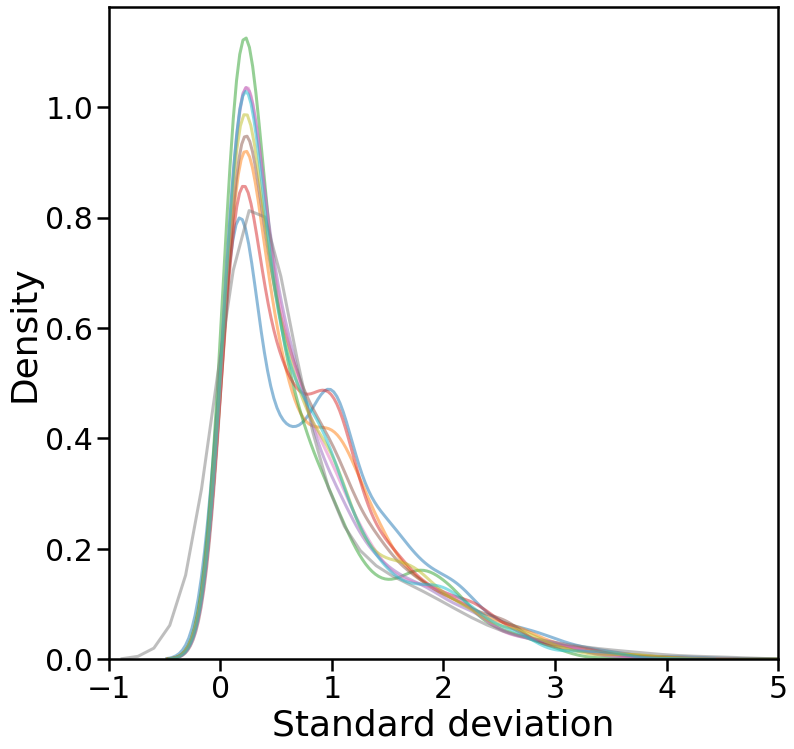
\includegraphics[width=0.5\linewidth]{../../result/mu_sigma_variance_plots/osw_log/osw_kde_qvalFiltered_pepFiltered_qbinned.png} & &%\includegraphics[width=0.3\linewidth]{} & 
        B 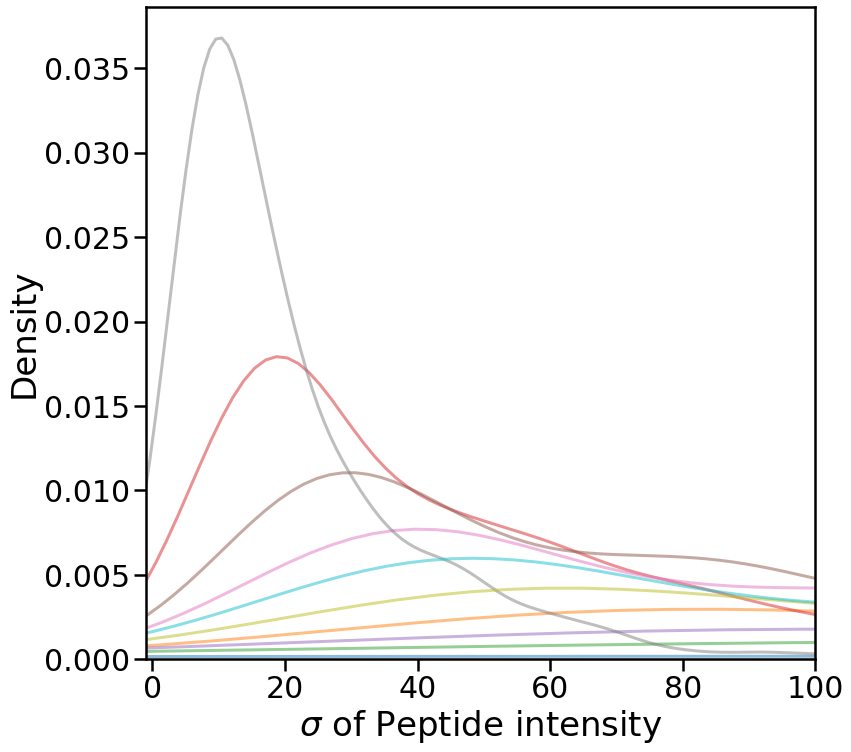
\includegraphics[width=0.5\linewidth]{../../result/mu_sigma_variance_plots/osw/osw_kde_nolog_qvalFiltered_pepFiltered_qbinned.png} & \\%\includegraphics[width=0.3\linewidth]{} \\ 
        C 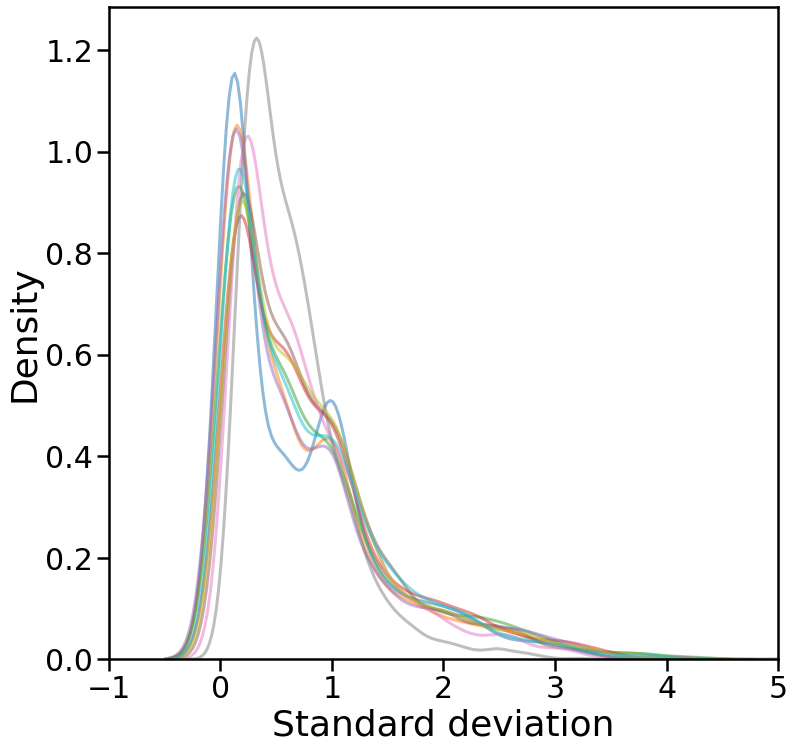
\includegraphics[width=0.5\linewidth]{../../result/mu_sigma_variance_plots/diann_log/diann_kde_qvalFiltered_pepFiltered_qbinned.png} & &%\includegraphics[width=0.3\linewidth]{} & 
    \end{tabular}
  \caption{{\bf Gaussian kernel density estimates of quantile binned peptide intensities.} We plotted the Gaussian kernel estimates of the quantile binned peptide intensities for (A-C) ID and (C-D) PS workflows. Approximately equal densities in the bins demonstrates the uniform offset in standard deviation across the intensity scale. \label{fig:mu_sigma_KDE_find_a_better_label}}
\end{figure}
\fi


% Please add the following required packages to your document preamble:


\begin{table}[hbt]
\centering
\begin{tabular}{llll}
\hline
        & Unfiltered & no\_shared & no\_shared\_IL\_equivalence \\ \hline
All     & 31 055     & 30 456     & 30 452                      \\
E. Coli & 4 391      & 4 306      & 4 306                       \\
Human   & 20 614     & 20 302     & 20 299                      \\
Yeast   & 6 050      & 5 848      & 5 847                       \\ \hline
\end{tabular}

  \caption{{\bf Protein count in the Uniprot FASTA protein database.} The database is a FASTA file with one protein sequence per gene for each species (UP000005640, UP000000625 and UP000002311. Acquired on 2021-06-16). The "no\_shared" filter is applied by splitting the protein sequences at amino acids "K" and "R" and keeping all the sequences with length $>$ 7 for each protein. We then mapped each sequence to all possible protein matchings and counted the how many proteins each split sequence was mapped to, and filtered so that each sequence only kept one protein match. Therefore, creating a database library with only one peptide sequence per protein. For the "no\_shared\_IL\_equivalence" all I are replaced by L before performing the filtering. \label{table:proteins_in_database}}

\end{table}



\subsubsection*{Comparison of statistical calibration}
\begin{figure}[hbt]
    \centering
    \centering
    \begin{tabular}{lclc} 
        A 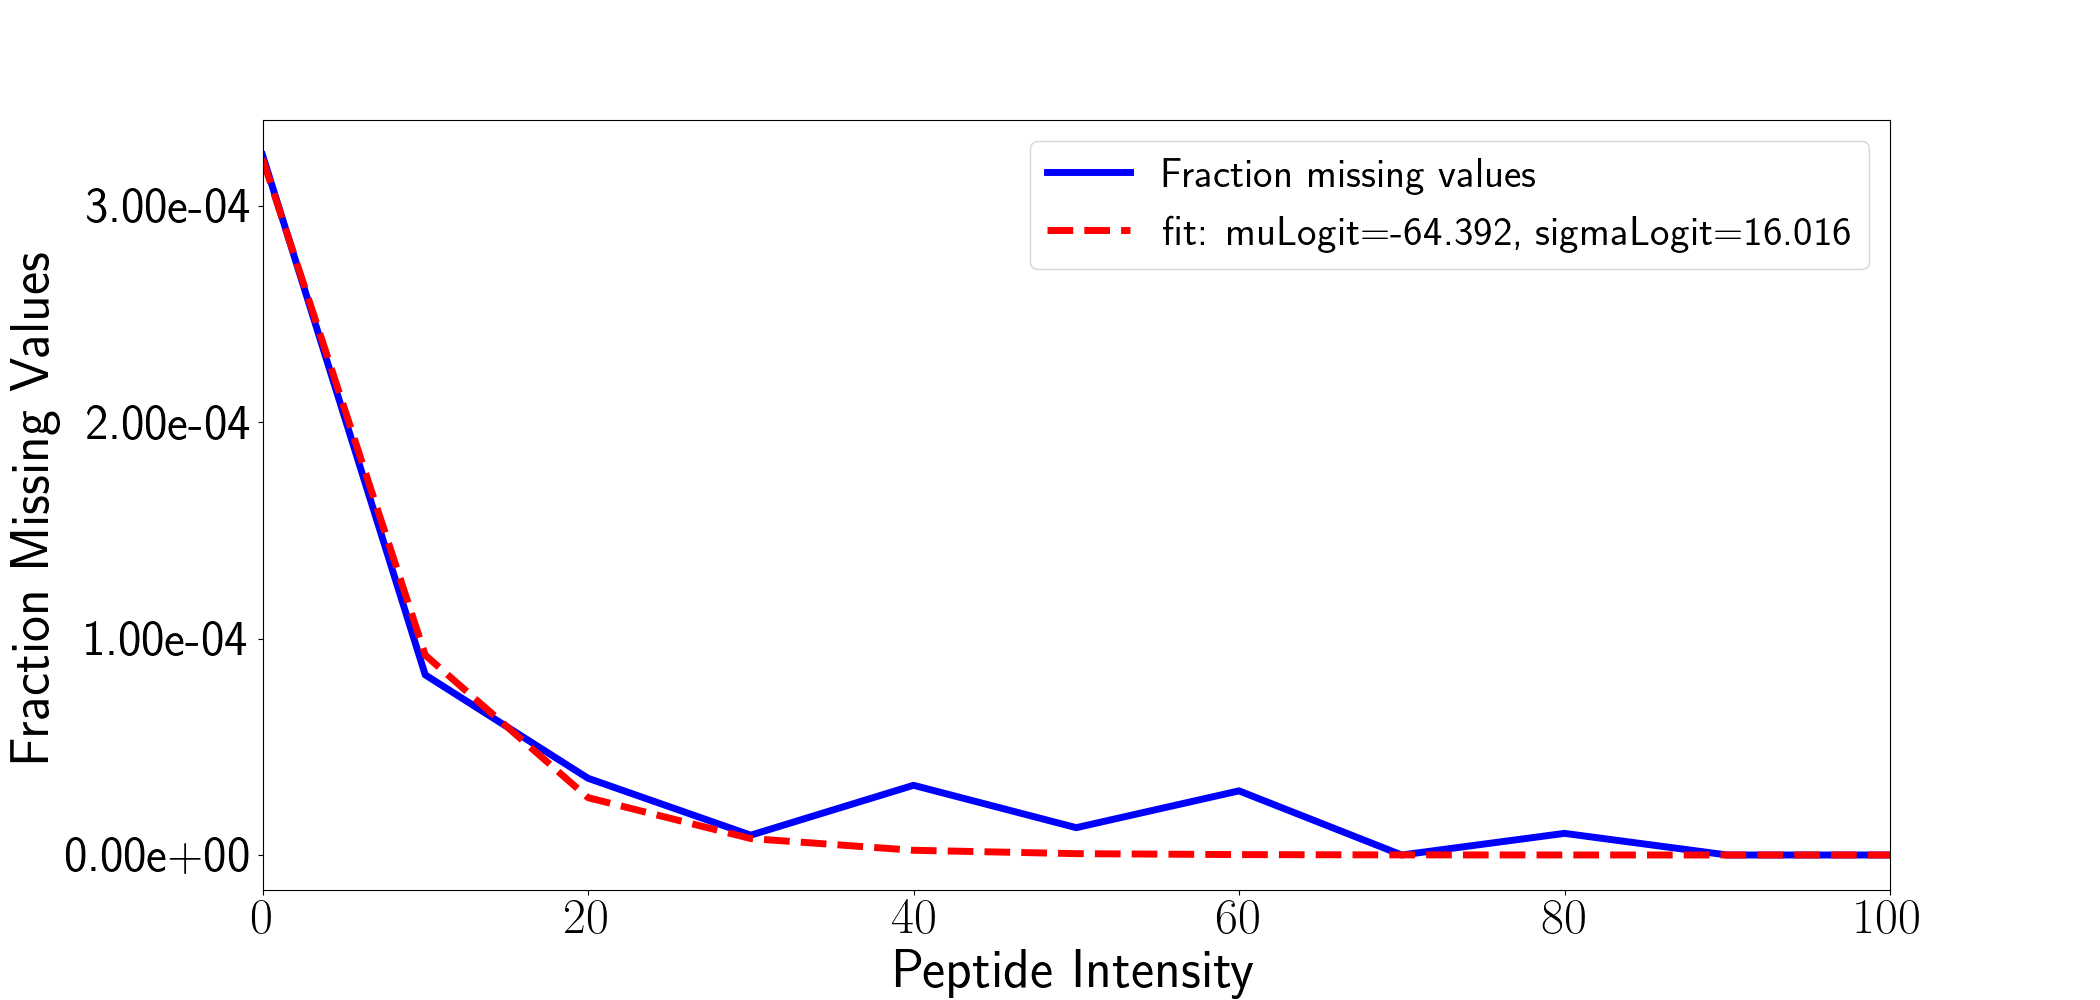
\includegraphics[width=0.5\linewidth]{../../result/report_plots_pipeline/fraction_missing_values_ID.png} & &%\includegraphics[width=0.3\linewidth]{} & 
        B 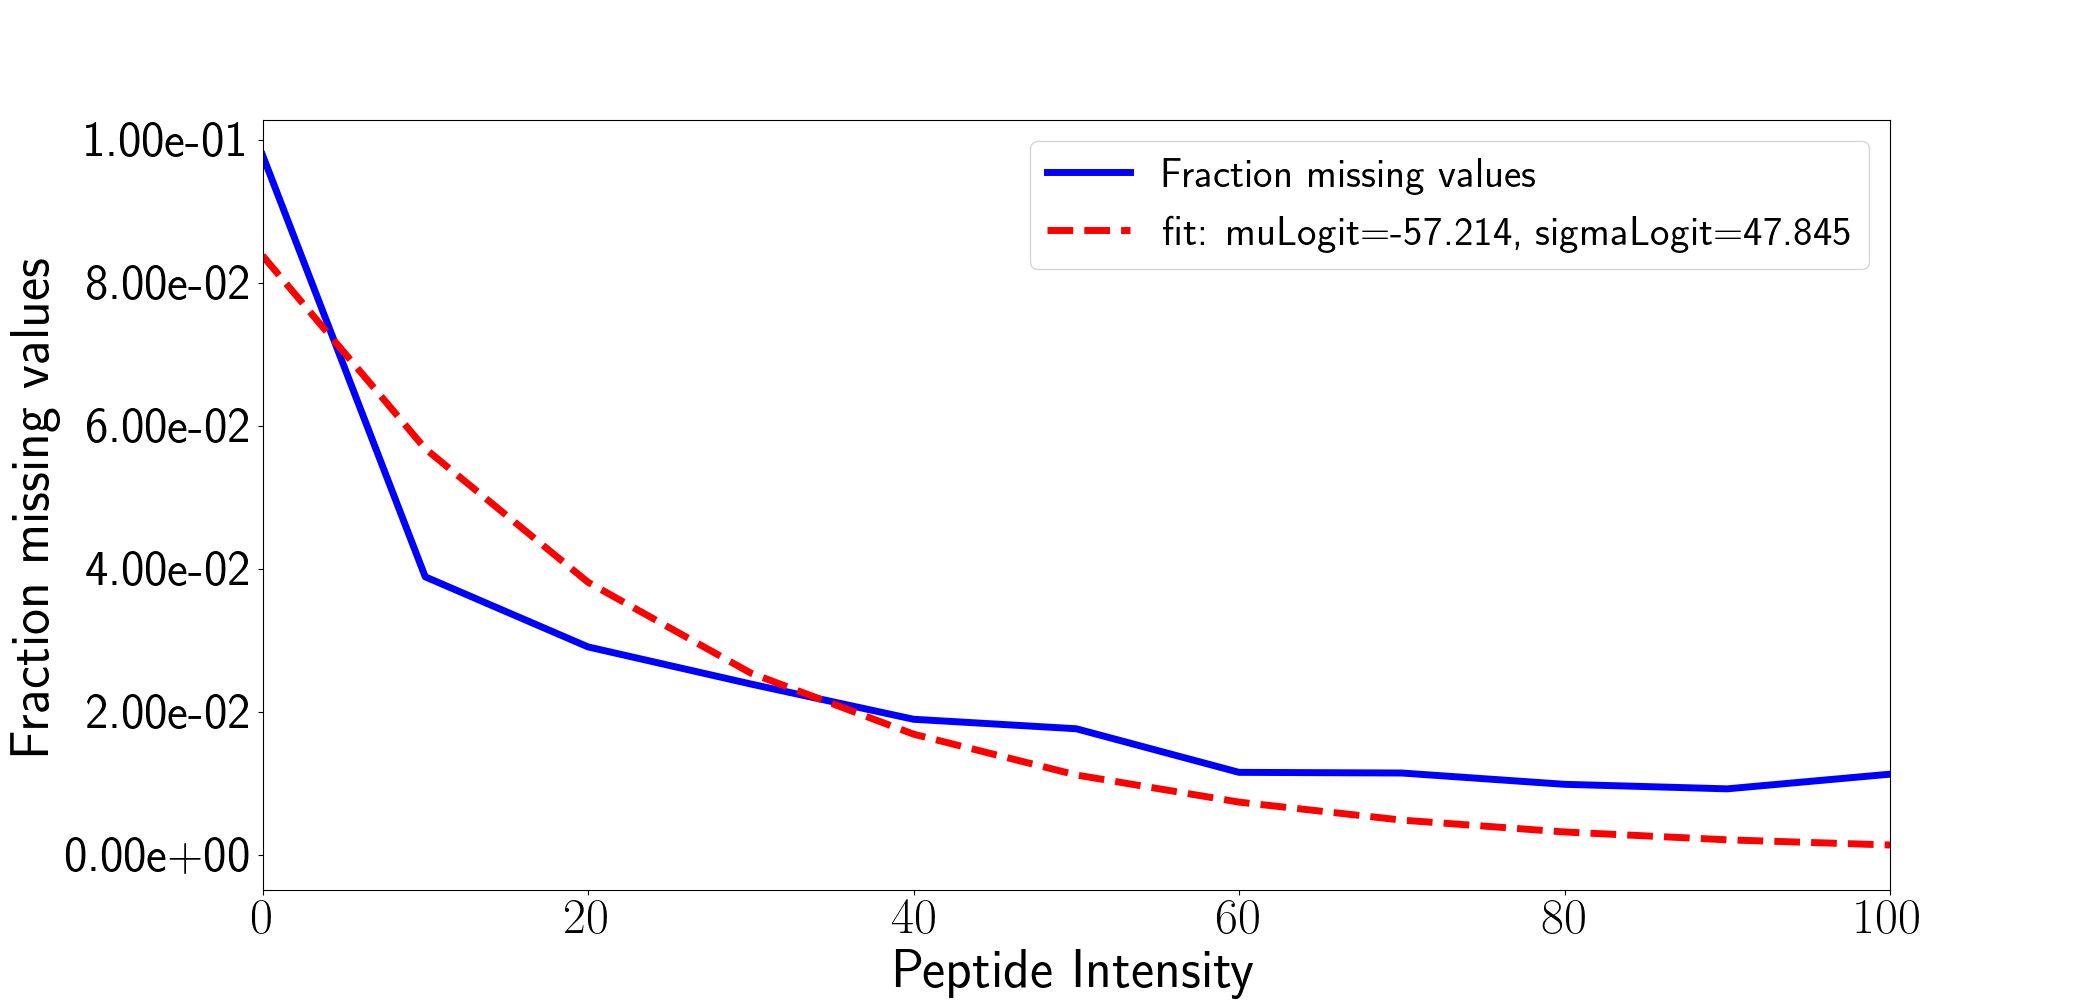
\includegraphics[width=0.5\linewidth]{../../result/report_plots_pipeline/fraction_missing_values_PS.png} & \\%\includegraphics[width=0.3\linewidth]{} \\ 
    \end{tabular}
    \caption{{\bf Comparison of actual missing values against fit to the censored normal distribution used in triqler.} We imputed the missing values as the mean of sample peptide intensities and used these imputed values to approximate the missingness for a given intensity. We binned the intensities to an arbitrary small range and plotted the fraction os missing values for each intensity range. A cubic spline fit was used to fit the values against the mentioned censored normal distribution for (A) SL pipeline  and (B) PS pipeline. \label{fig:fraction_missing_values}}

\end{figure}


\subsubsection*{Comparison of reported protein count}
\begin{figure}[hbt]
    \centering
    %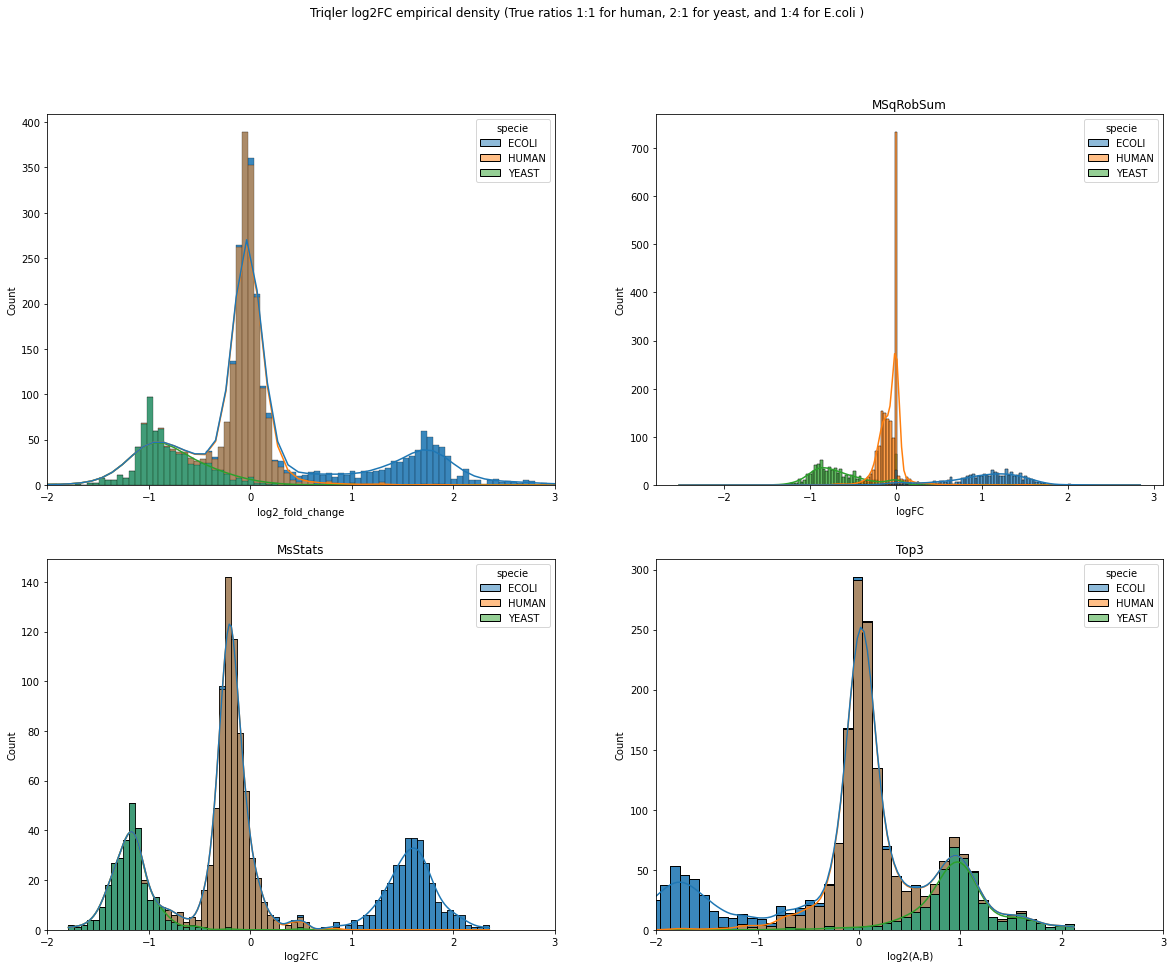
\includegraphics[width=16cm]{../../result/2021-08-13_docs_plots/intensity_plot.png}
    \begin{tabular}{lclc} 
        A & 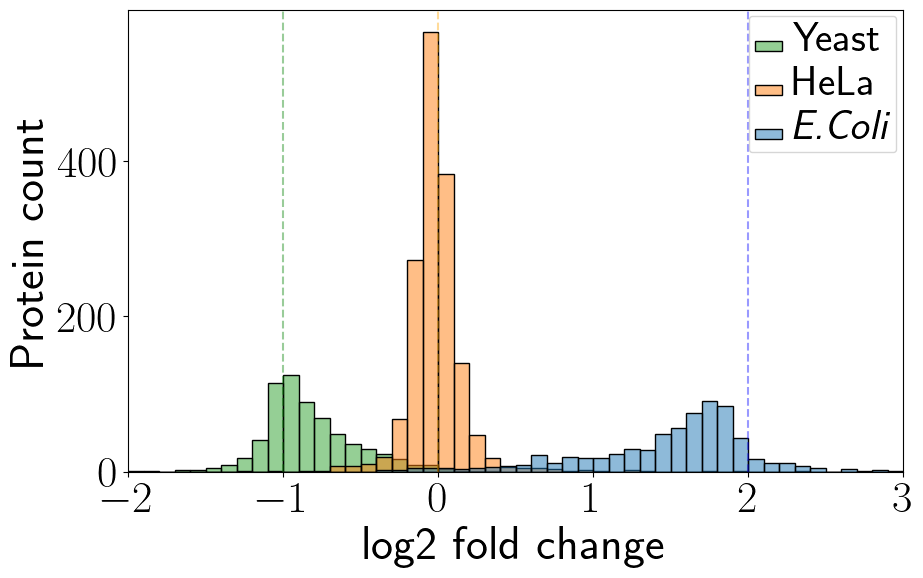
\includegraphics[width=0.4\linewidth]{../../result/report_plots_pipeline/histogram_ID_triqler.png} & 
        E & 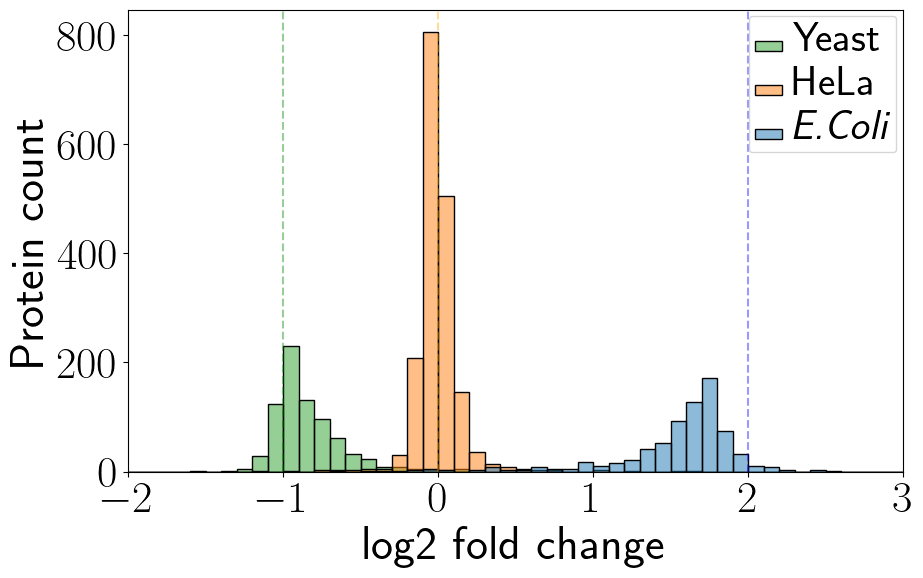
\includegraphics[width=0.4\linewidth]{../../result/report_plots_pipeline/histogram_PS_triqler.png} \\ 
        B & 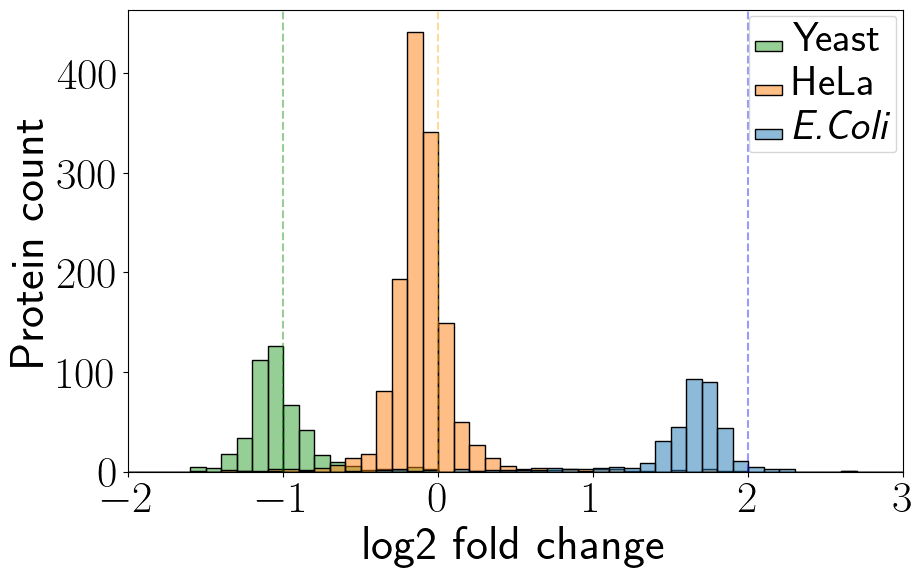
\includegraphics[width=0.4\linewidth]{../../result/report_plots_pipeline/histogram_ID_msqrob2.png} & 
        F & 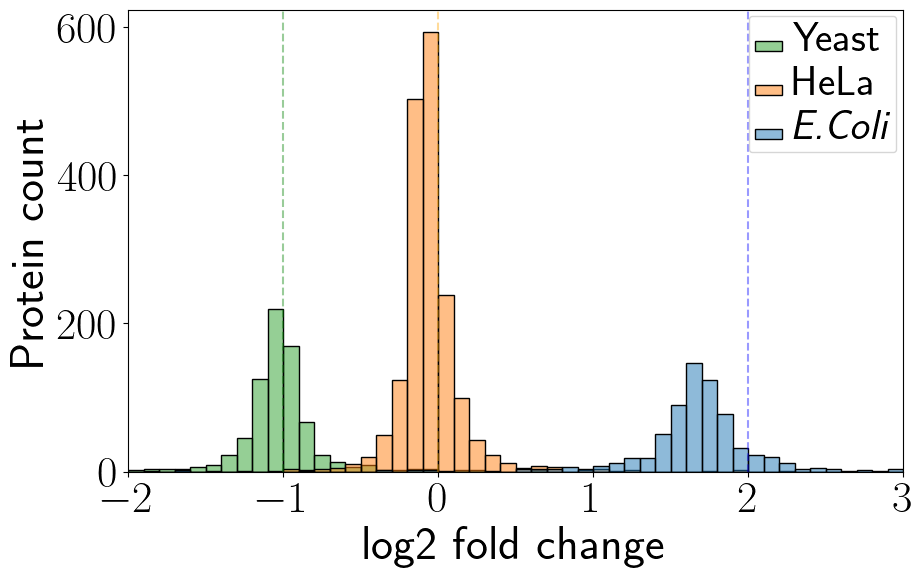
\includegraphics[width=0.4\linewidth]{../../result/report_plots_pipeline/histogram_PS_msqrob2.png} \\ 
        C & 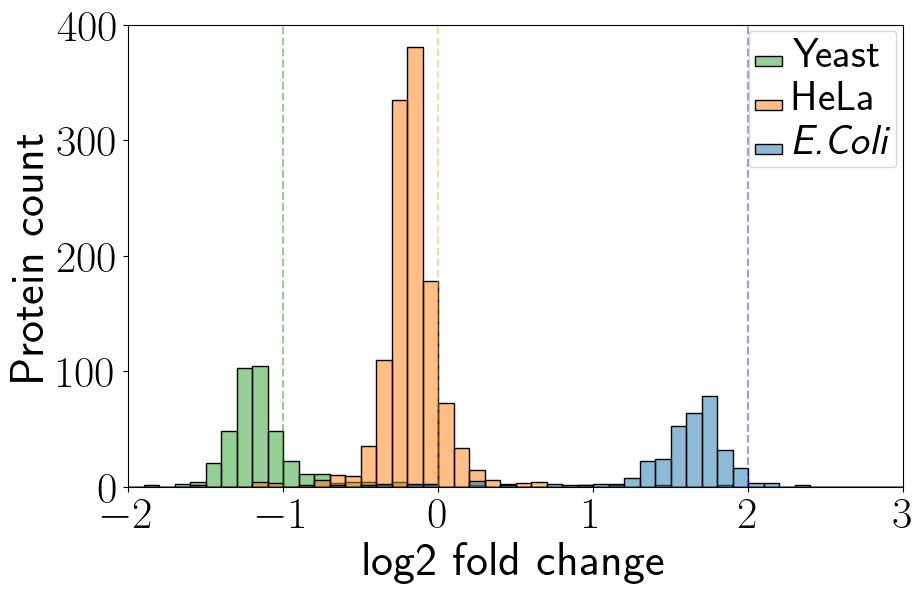
\includegraphics[width=0.4\linewidth]{../../result/report_plots_pipeline/histogram_ID_msstats.png} & 
        G & 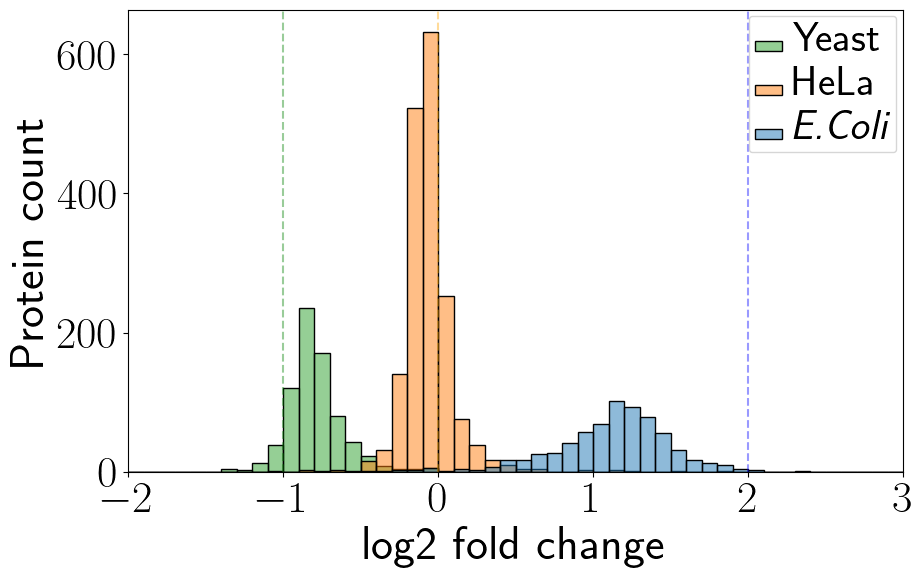
\includegraphics[width=0.4\linewidth]{../../result/report_plots_pipeline/histogram_PS_msstats.png} \\ 
        D & 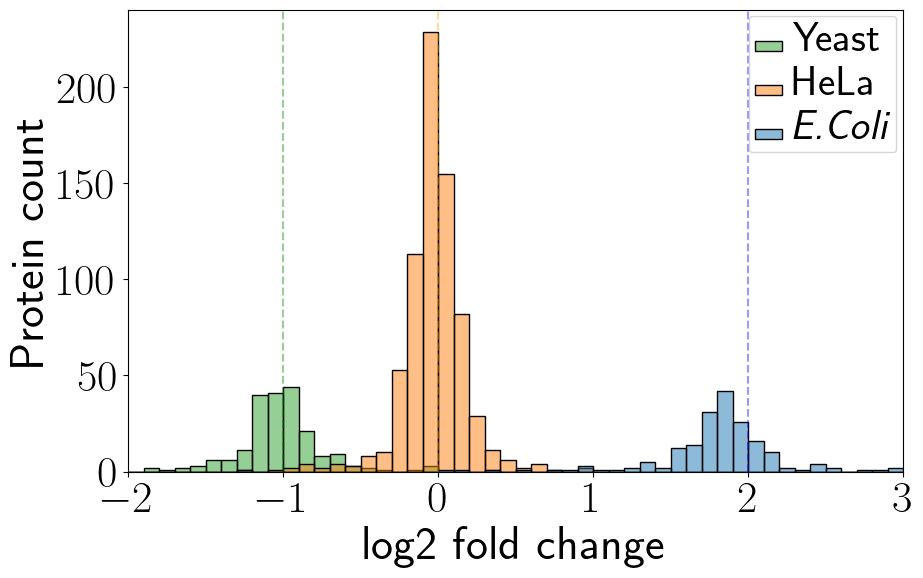
\includegraphics[width=0.4\linewidth]{../../result/report_plots_pipeline/histogram_ID_top3.png} &
        H & 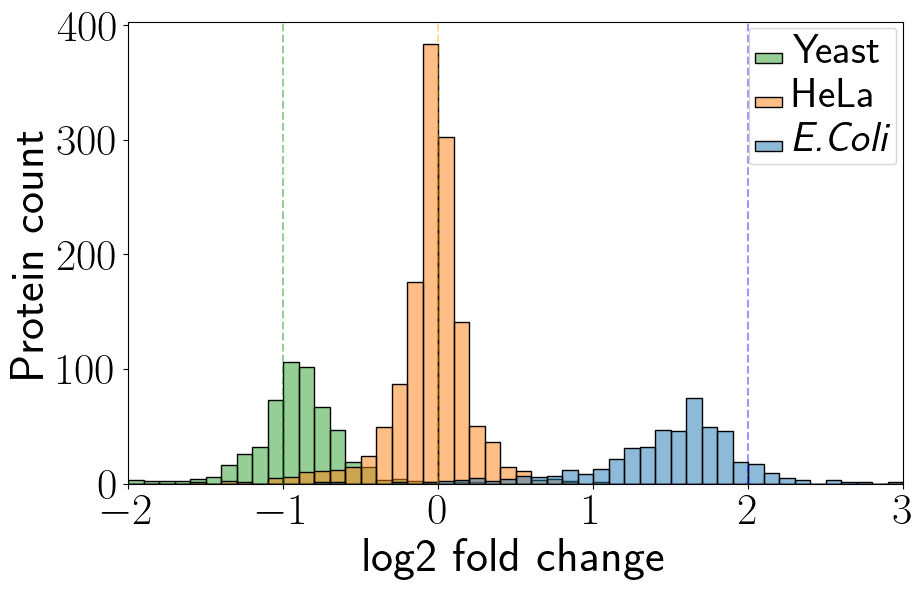
\includegraphics[width=0.4\linewidth]{../../result/report_plots_pipeline/histogram_PS_top3.png} 
    \end{tabular}
    \caption{{\bf Comparison of reported fold change distributions.} We used protein data from (A-D) ID and (E-H) PS pipelines as generated by 
    (A,E) Triqler, (B,F) MSqRob2, (C,G) MSstats, and (D,H) Top3. \label{fig:fc_histogram_supplement}}
\end{figure}

\subsubsection*{Protein-level results}
\begin{figure}[hbt]
    \centering
    %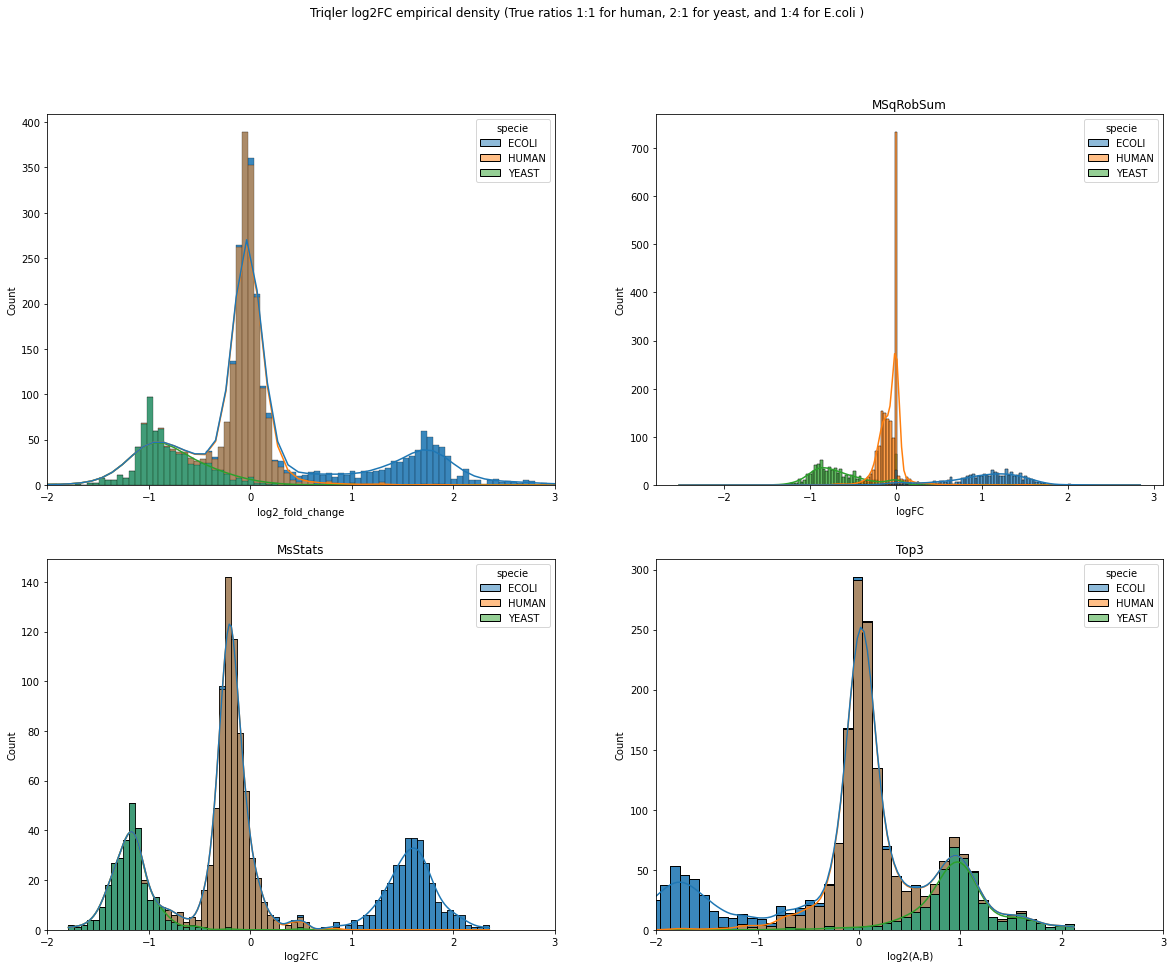
\includegraphics[width=16cm]{../../result/2021-08-13_docs_plots/intensity_plot.png}
    \begin{tabular}{lclc} 
        A & 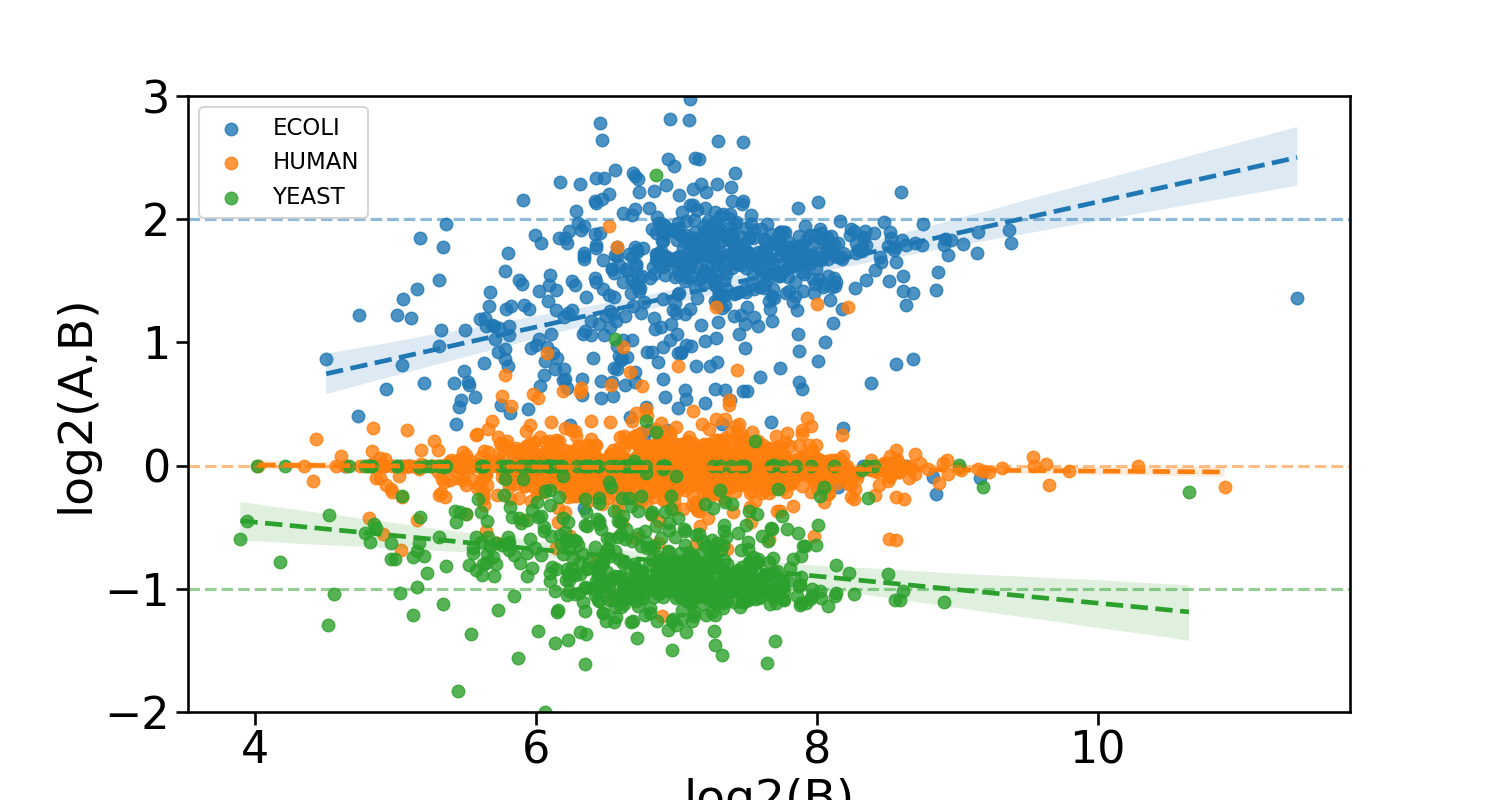
\includegraphics[width=0.4\linewidth]{../../result/report_plots_pipeline/scatter_ID_triqler.png} & 
        E & \includegraphics[width=0.4\linewidth]{../../result/report_plots_pipeline/scatter_PS_triqler.png} \\ 
        B & \includegraphics[width=0.4\linewidth]{../../result/report_plots_pipeline/scatter_ID_msqrob2.png} & 
        F & \includegraphics[width=0.4\linewidth]{../../result/report_plots_pipeline/scatter_PS_msqrob2.png} \\ 
        C & \includegraphics[width=0.4\linewidth]{../../result/report_plots_pipeline/scatter_ID_msstats.png} & 
        G & \includegraphics[width=0.4\linewidth]{../../result/report_plots_pipeline/scatter_PS_msstats.png} \\ 
        D & \includegraphics[width=0.4\linewidth]{../../result/report_plots_pipeline/scatter_ID_top3.png} &
        H & \includegraphics[width=0.4\linewidth]{../../result/report_plots_pipeline/scatter_PS_top3.png} 
    \end{tabular}
    \caption{{\bf Protein level results} from (A-D) ID and (E-H) PS pipelines as generated by 
    (A,E) Triqler, (B,F) MSqRob2, (C,G) MSstats, and (D,H) Top3. \label{fig:fc_scatter_supplement}}
\end{figure}



\subsubsection*{Comparison of statistical calibration}
\begin{figure}[hbt]
    \centering
    \centering
    \begin{tabular}{lclc} 
        A \includegraphics[width=0.4\linewidth]{../../result/report_plots_pipeline/calibration_ID_0.png} & &%\includegraphics[width=0.3\linewidth]{} & 
        C \includegraphics[width=0.4\linewidth]{../../result/report_plots_pipeline/calibration_ID_0.51.png} & \\%\includegraphics[width=0.3\linewidth]{} \\ 
        B \includegraphics[width=0.4\linewidth]{../../result/report_plots_pipeline/calibration_PS_0.png} & &%\includegraphics[width=0.3\linewidth]{} & 
        D \includegraphics[width=0.4\linewidth]{../../result/report_plots_pipeline/calibration_PS_0.51.png} & \\%\includegraphics[width=0.3\linewidth]{} \\ 
    \end{tabular}
  \caption{{\bf Comparison of calibration of the compared summarization methods.} We plotted the fraction of reported differentially abundant HeLa proteins as a function of $q$~value for (A,C) ID pipeline and (B,D) PS pipeline. (A,C) is non FC-thresholded and (C,D) is FC-thresholded at 0.51. \label{fig:frac_hela_vs_fdr}}
\end{figure}



\end{document}
